% this file is called up by thesis.tex
% content in this file will be fed into the main document

\chapter{Evaluation}\label{ch:evaluation} % top level followed by section, subsection


% ----------------------- paths to graphics ------------------------

% change according to folder and file names
\ifpdf
    \graphicspath{{figures/PNG}}
\else
    \graphicspath{{7/figures/EPS/}{7/figures/}}
\fi


% ----------------------- contents from here ------------------------
% 
In this section, the experimental results are presented.
%First a baseline of RDMA performance on DAS is given.
%This will be used to compare a KV store use case to maximum performance that can be achieved on DAS.
The RDMA transportation types are compared within and against the baseline TCP implementation.
Throughput and latency are mainly used to analysis the scalability of these transportation types.
The same raw data is used for both measurements, thus can be put alongside each other.

In short, the results show:
\begin{itemize}
    \item Throughput reaches an equilibrium with all transportation types up to 30 clients.
    UD performs best, with a maximum throughput of roughly 400 kilo-tasks/sec.
    Further details are given in section \ref{sec:throughput-analysis}.
    \item Latency increases across all transportation types, with increased number of clients.
    Results are inversely comparable to throughput, again with UD performing best, with a latency of roughly 64 $\mu$sec at 30 clients.
    Section \ref{sec:latency:analysis} delves deeper.
\end{itemize}

To recall the benchmarking setup:
Ten million tasks are divided equally between \textit{n}-clients.
A task is defined as a request and response, and are equal to two operations.

\section{Throughput analysis}\label{sec:throughput-analysis}
We compare the average throughput between TCP, RC, and UD with up to 30 clients.
From figure \ref{fig:throughput-30}, the maximum average throughput is observed to be roughly 205 kilo-tasks/sec for TCP, 251 kilo-tasks/sec for RC, both at 30 clients, and 399 kilo-tasks/sec for UD at 25 clients.
RC shows a mere 22.8\% maximum improvement over TCP.
UD in turn offers a significant gain of 94.8\% over TCP.
\begin{figure}
    \centering
    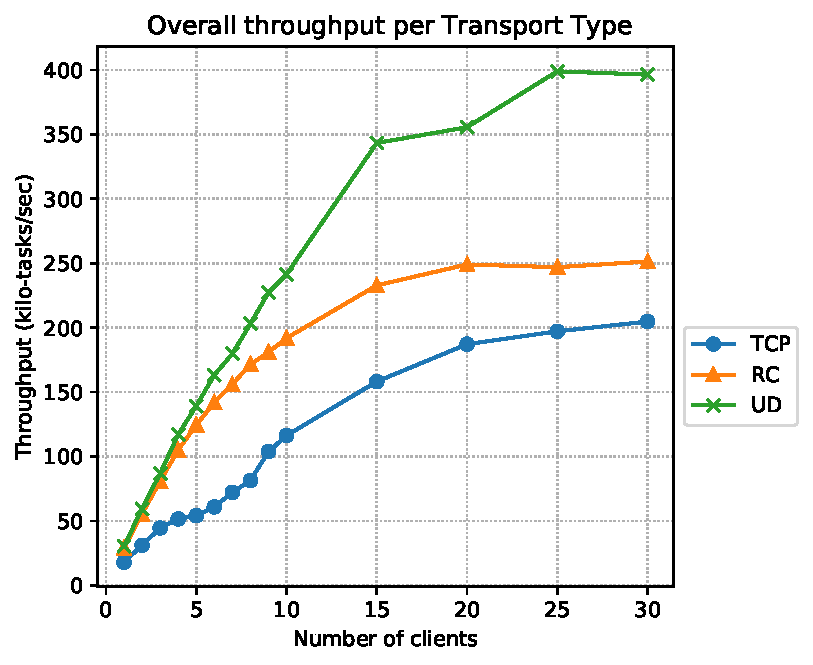
\includegraphics[height=8cm]{figures/PDF/Throughput_30}
    \caption{Throughput of clients executing 10 million operations}
    \label{fig:throughput-30}
\end{figure}

\subsection{Scalability rate}\label{subsec:scalability-rate}
It can be observed from figure \ref{fig:throughput-30} that all transportation types scale up to roughly 20 clients before settling.
UD outperforms the other types, in both throughput and initial rate of scalability.
A near linear scalability rate can be seen in the first 15 clients for UD.
This is due the addition of threads for every new client.
Since all these threads are actively working for all clients, this linear increase is to be expected.
For the first 10 clients, UD increases its throughput by 23.4 kilo-tasks/sec per additional client.
Compare this with 18.1 for RC and 10.9 kilo-tasks/sec for the baseline TCP.
This shows strong scalability for UD with small number of clients.
It is unclear from this graph if UD continues to scale beyond 30 clients.

\subsection{Similarities between RC and TCP}
It can also be seen in figure \ref{fig:throughput-30} that RC is similar to TCP in scalability.
With both being a connection oriented protocol, each server thread being tied to a client, it shows similar performance.
The benefits of RDMA do reflect in these results, with the throughput of RC being on average 59.7 kilo-tasks/sec above TCP.
Both protocol stabilizing after roughly 20 clients, with less than 5\% change for TCP and less than 2\% for RC.

%\subsection{Fairness between clients}
%TODO GENERATE GRAPH FOR THIS

\section{Latency analysis}\label{sec:latency:analysis}
An important factor to KV store is their quick response time, and therefore this should ideally scale similarly, preferably better, than throughput.
RDMA offers fast response time due to the lack of CPU and kernel involvement.
To see how this is translated per transportation type, the average latency of all 10 million tasks were measured, from request sent to response received.
Results can be seen in figure \ref{fig:latency-30}.
Along with the average latency, the first and third quartile are shown, to analyze the variation of latencies.

\begin{figure}
    \centering
    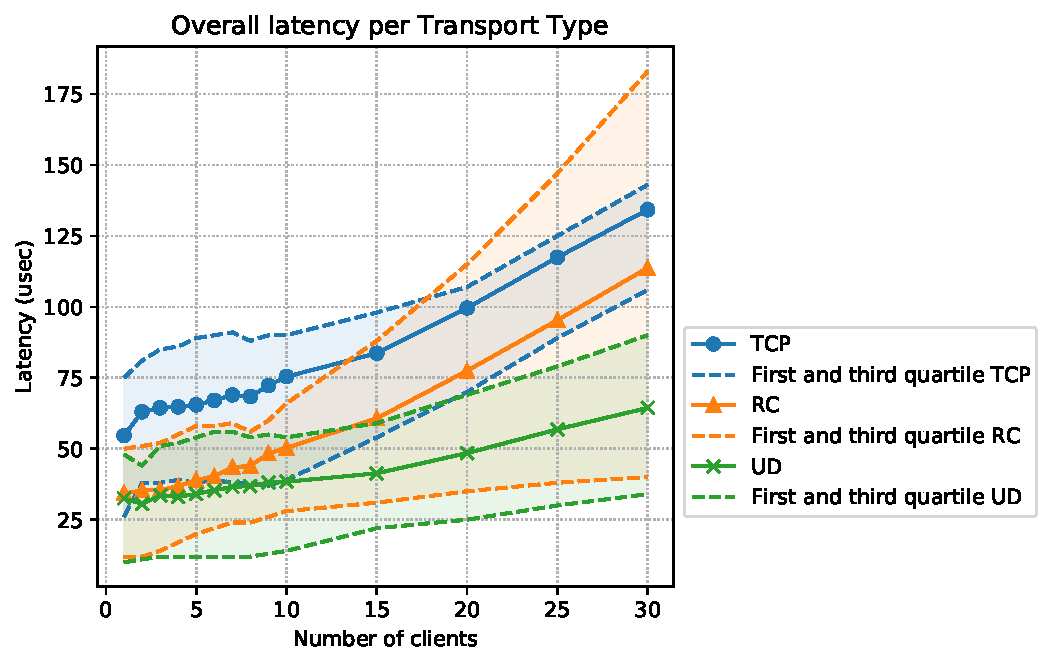
\includegraphics[width=\columnwidth]{figures/PDF/Latency_avg_30}
    \caption{Latency of clients executing 10 million operations}
    \label{fig:latency-30}
\end{figure}

The latency between protocols is an inverse reflection of the throughput graph, scaling and overall performance.
Similarly, TCP performed worst, with an average latency of 134.2 $\mu$sec at 30 clients.
RC hits an average of 113.7 $\mu$sec, also at 30 clients.
UD again performing best, reaching 64.4 $\mu$sec on average.
This is an order of magnitude more than has been found in FaSST\cite{kalia2016fasst}, HERD\cite{kalia2014using}, and what should be theoretically possible.
This could be due to lock contention with shared QP, and poor performance of KV store.
A further examination of this could support this.

Similarly to throughput, UD scales relatively well, while RC and TCP scale linearly.
A near uniform latency for the first 15 clients, afterwards a gradual slope, compared to TCP and RC.

\subsection{Variation from average}
In figure \ref{fig:latency-30} the variation is given in form of first and third quartile.
It can be seen that TCP and UD have a constant, a small, variation.
TCP is skewed towards higher latencies at 30 clients, while UD, and RC, stay normally distributed throughout.
RC has a rapidly increasing variation.
This is concerning for scalability and consistency, and could possibly be due to context switching.

\subsection{All 30 clients and per operation latency}\label{subsec:all-30-clients-and-per-operation-latency}

\begin{figure}
    \centering
    \subfigure[TCP] {
        \centering
        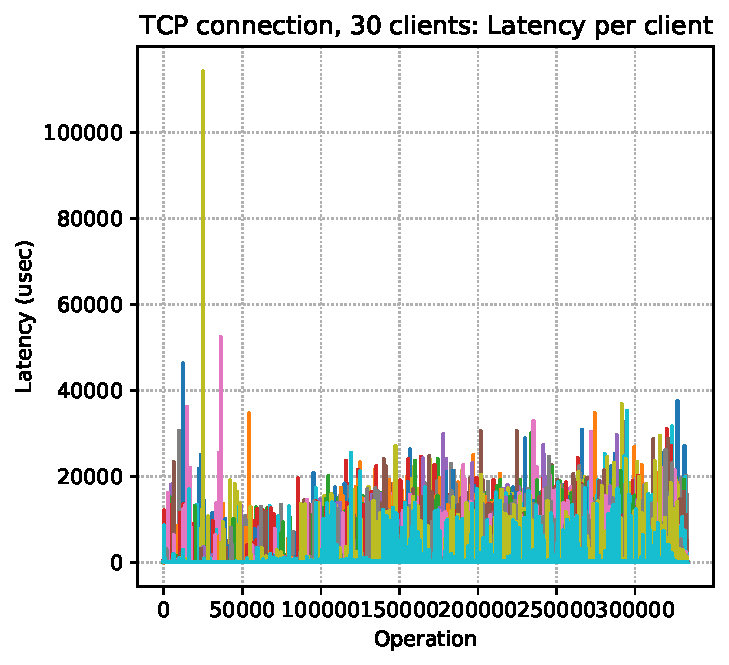
\includegraphics[width=0.47\columnwidth]{figures/PDF/TCP_Latency_30}
        \label{fig:tcp_latency_30}
    }
    \subfigure[RC] {
        \centering
        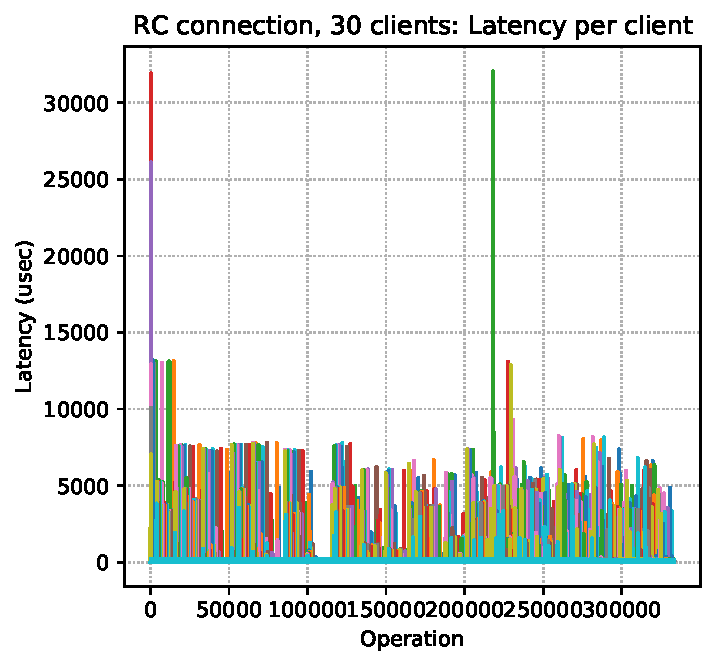
\includegraphics[width=0.47\columnwidth]{figures/PDF/RC_Latency_30}
        \label{fig:rc_latency_30}
    }
    \subfigure[UD] {
        \centering
        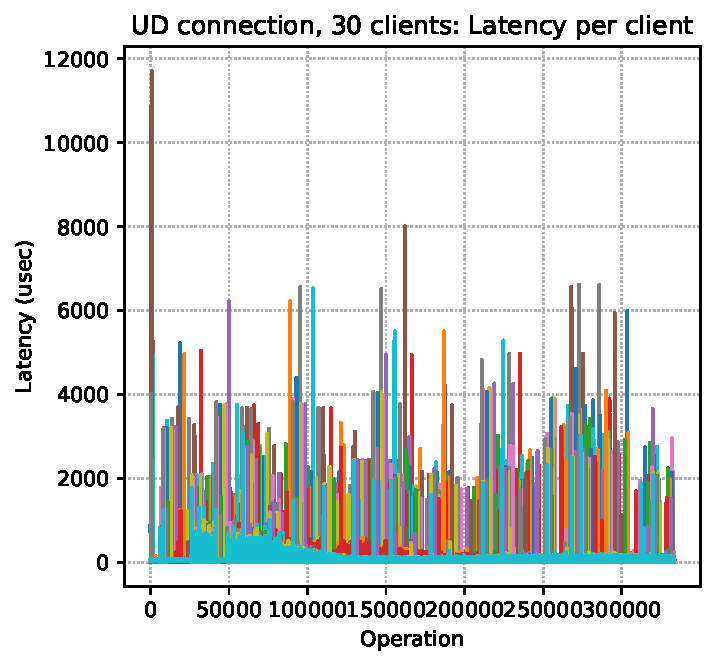
\includegraphics[width=0.47\columnwidth]{figures/PDF/UD_Latency_30}
        \label{fig:ud_latency_30}
    }
    \caption{Structure for response with accommodated response codes}
    \label{fig:latencies_30}
\end{figure}


Figure \ref{fig:latencies_30} delves deeper into the details of the latency outliers that are present.
Note on the scale, not similar between protocols, and compared to figure \ref{fig:latency-30}.
These outliers are the extreme outliers.
TCP and RC see spikes up to 114185 $\mu$sec, or 114.2ms, and 32046 $\mu$sec, or 32.05ms.
UD on the other only spikes to a maximum of 11702 $\mu$sec, or 11.7ms.

\subsection{RDMA multiple QP's causing cache misses and context switching}
In section \ref{subsec:transportation-types} the issue with holding multiple QP's within the RNIC, has been discussed.
The RNIC needs to perform context switching when changing QP.
As the number of QP's increase, like with connection oriented transport types, the number of context switches needed increases.
Along this, the chance of cache misses are also increased.
This decreases the performance, with increased latency, and in throughput as shown here.
With context switching, a large delay occurs, and harms the performance per client, but also of the overall network.
For this reason, for large number of clients, a one-to-one QP is not advisable.

\subsubsection{Cache misses as increased variation for RC}
Furthermore, cache misses occur more often at the starting phase of KV store operations, as can be seen in section \ref{fig:rc_latency_30} above.
RC has consistently higher latency (0.75ms) for some clients at the start.
Initially it was thought to be retransmissions, however for this was set to 67.1ms.
Since this only occurs to some clients, and not all, this could be a result from the aforementioned context switching and RNIC cache misses.
At the start of operations, worker threads are operating in sync.
This would result in RNIC processing multiple WR's concurrently.
Some QP's will be cached and experience little cache misses throughout the starting phase, while others would encounter cache misses repeatedly.
Once threads are out of sync and KV store operation latency increases (due to the increasing size of the hash table), the cache misses will occur for all QP's.
This can be seen in figure \ref{fig:rc_latency_30}, as the latency in the final phase is randomized and less constant, compared to the starting phase.

With cache misses, latency per client varies, as some QP's would require further lookup after cache miss.
This effect can be seen in figure \ref{fig:latency-30}, as increasing number of clients, and therefore QP's, increases the variation dramatically.
Further investigation into cache misses would support these claims, this has not been done for this thesis.

% ---------------------------------------------------------------------------
% ----------------------- end of thesis sub-document ------------------------
% ---------------------------------------------------------------------------